\section{Analyse der Struktur}
In diesem Kapitel wird beschrieben, wie Kräfte und Spannungen im Solar Butterfly, entstehend durch verschiedene Lastfälle, vereinfacht berechet werden. Es wird erläutert welche Annahmen und Idealisierungen getroffen werden und wie bei den Berechnungen vorgegangen wird. Weiter werden die Berechnungen bezüglich den erlangetn Resultaten und ihrer Aussagekraft Beurteilt.\\
Die Berechnungen wurden mit einer Excel-Tabelle gemacht, welche im elektronischen Anhang [ANHANG] einsehbar ist. In ihr sind die exakten Resultate sowie der detailiertere Lösungsweg zu finden.

\paragraph{Massenverteilung}\mbox{}\\
Die grössten Belastungen, welchen der Solar Butterfly ausgesetzt wird, entstehen aufgrund der Trägheitskräfte welche durch Beschleunigungen entstehen. Aus diesem Grund wird die Massenverteilung des Solar Butterflys genauer betrachtet. Für die festlegung der Massenverteilung wird angenommen, dass die in der Anforderungsliste definierte Maximalmasse von 3000 kg erreicht wird. Die besagte Masse wird auf insgesamt sechs Bereiche aufgeteilt; Deichsel (Bereich 0-1), Küche (1-2), Hauptkörper (2-3), Bad (3-4) und die beiden Träger A (2) und B (3). Die Massenverteilung wurde mit der Hilfe des GEWICHTSEXCEL aus der Arbeit von \emph{Huber} (Anhang [ANHANG]) abgeschätzt und ist in der Abbildung \ref{Massenverteilung} grafisch dargestellt.

\begin{center}
  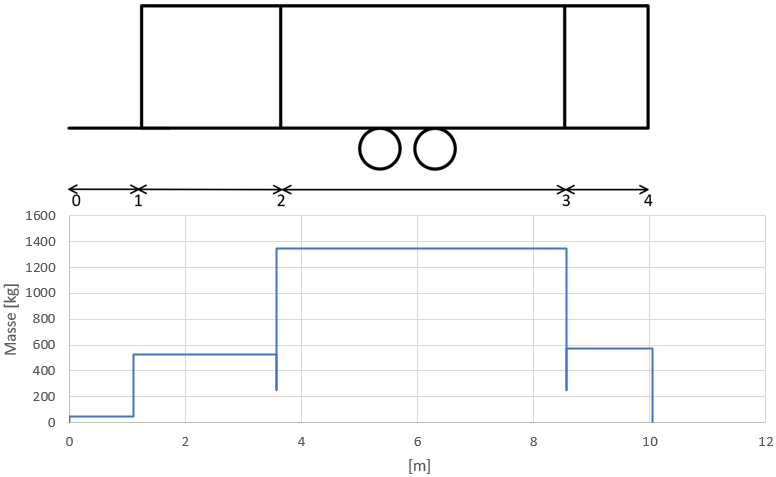
\includegraphics[width=0.8\textwidth]{04_Figures/Massenverteilung.png}
  \captionof{figure}{Massenverteilung über die Bereiche}
  \label{Massenverteilung}
\end{center}

\subsection{Vertikale Beschleunigung}
\label{1.1 Vertikale Beschleunigung}
  \paragraph{Idealisierung}\mbox{}\\
  Um die Kräfte und Spannungen in der Struktur, welche aufgrund der vertikalen Beschleunigung (Lastfall \emph{1.1 Vertikale Beschleunigung}) entstehen, berechnen zu können, wird der Solar Butterfly als Biegebalken mit dem in der Abbildung \ref{1.1 Idealisierter Querschnitt} dargestelltem vollidealisiertem Querschnitt idelaisiert. \emph{A\_Dach} und \emph{A\_Chassis} stehen dabei für die Querschnittsflächen der Profile. \emph{z\_Dach} und \emph{z\_Chassis} stehen für den Abstand der Profile zum Flächenschwerpunkt. Das Profil des Chassis ist vom Hersteller vorgegeben und muss in der Grobauslegung nicht dimensioniert werden. Für die Längsträger des Daches wird für eine erste Iteration der Berechnungen ein 50x25-Rechteckprofil mit einer Wandstärke von 3 mm verwendet. Dieser Profilquerschnitt wurde aufgrund den Erkenntnissen, welche im Kapitel REF erlangt wurden, gewählt. Die Lagerung des Biegebalkens ist in der Abbildung \ref{1.1 Lagerung} dargestellt.

  \begin{figure}[!ht]
    \centering
      \begin{subfigure}{.4\textwidth}
        \centering
        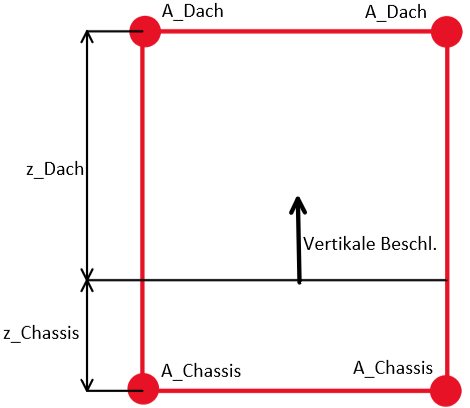
\includegraphics[width=\linewidth]{04_figures/1.1 Querschnitt.png}
        \caption{Idealisierter Querschnitt}
        \label{1.1 Idealisierter Querschnitt}
      \end{subfigure}%
      \begin{subfigure}{.6\textwidth}
        \centering
        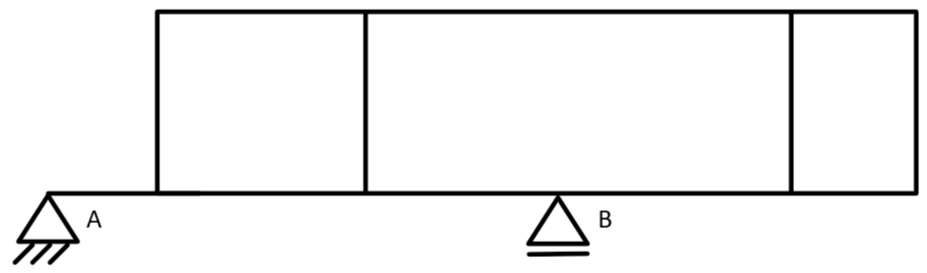
\includegraphics[width=\linewidth]{04_figures/1.1 Lagerung.png}
        \caption{Lagerung des idealisierten Solar Butterfly}
        \label{1.1 Lagerung}
      \end{subfigure}%
    \caption{Idealisierung des Solar Butterfly für den Lastfall der vertikalen Beschleunigung}
  \label{1.1 Idealisierung}
  \end{figure}

  \paragraph{Querkraft- und Biegemomentenverlauf}\mbox{}\\
  Aus der Massenverteilung und der vertikalen Beschleunigung können die Streckenlasten pro Abschnitt, die Gewichtskräfte der Träger A und B sowie die Lagerreaktionen berechnet werden. Aus ihnen können durch integration wiederum der Querkraft- und Biegemomentenverlauf berechnet werden, welche in der Abbildung \ref{1.1 QM} dargestellt sind.

  \begin{figure}[!ht]
    \centering
      \begin{subfigure}{.5\textwidth}
        \centering
        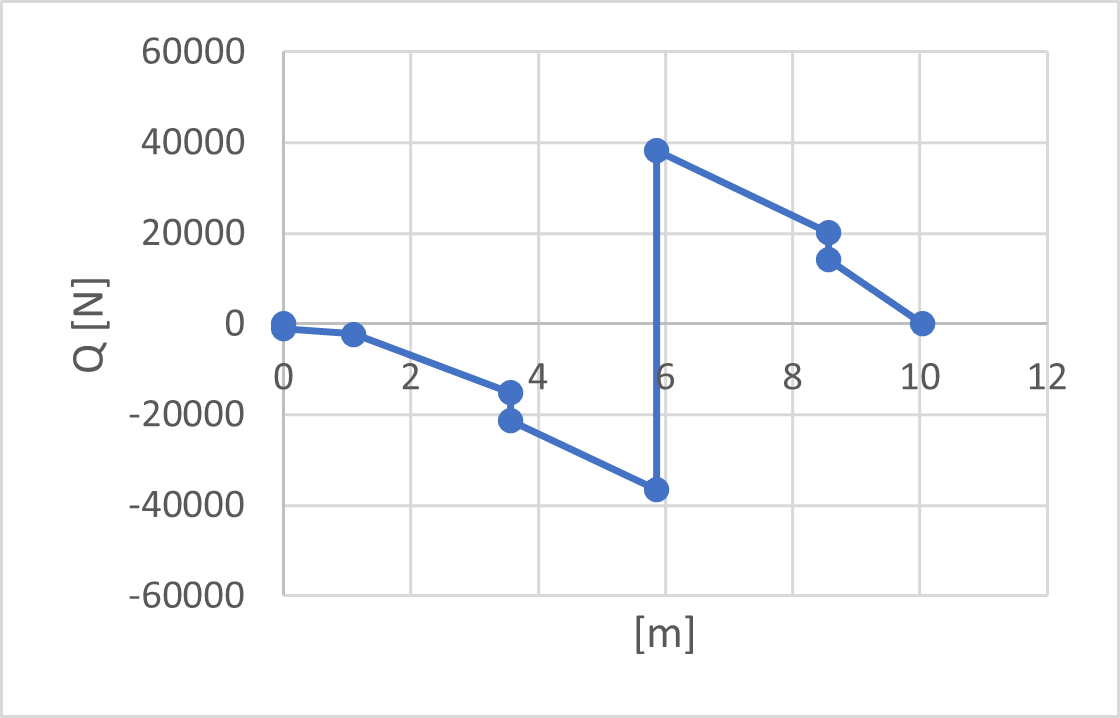
\includegraphics[width=.98\linewidth]{04_figures/1.1 Q.png}
        \caption{Querkraftverlauf}
        \label{1.1 Q}
      \end{subfigure}%
      \begin{subfigure}{.5\textwidth}
        \centering
        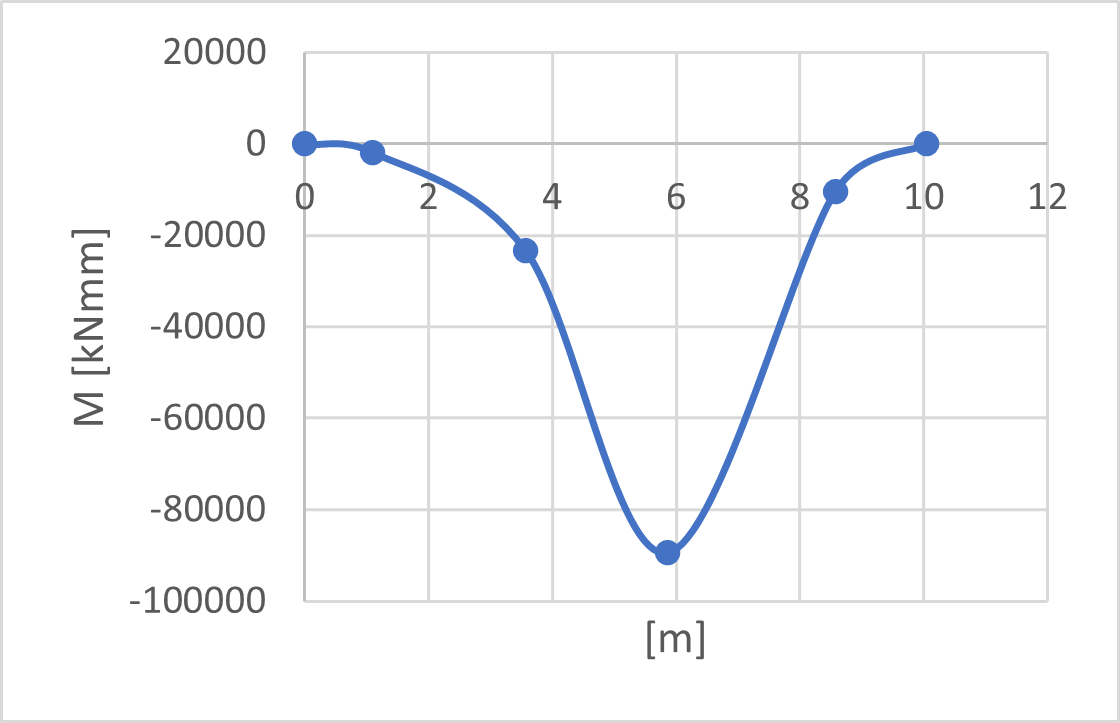
\includegraphics[width=.98\linewidth]{04_figures/1.1 M.png}
        \caption{Biegemomentenverlauf}
        \label{1.1 M}
      \end{subfigure}%
    \caption{Querkraft- und Biegemomentenverlauf}
  \label{1.1 QM}
  \end{figure}

  \paragraph{Spannungen und Kräfte}\mbox{}\\
  Da die Profile im Dach aus Aluminium sind, das Chassis jedoch aus Stahl, und daher unterschiedliche Steifigkeiten aufweisen, können die Spannungen nicht mit dem Widerstandsmoment, sondern müssen über die Biegesteifigkeit berechnet werden. Die Biegesteifigkeit ergibt sich durch die Gewichtung der Widerstandsmomente mit der Steifigkeit des jeweiligen Profiles (Formel \ref{eq:1}). Die Spannungen in den Profilen können wiederum mit der Formel \ref{eq:2} berechnet werden.

  \begin{equation}
    \label{eq:1}
      \overline{EI}_y = \sum A_i \cdot y_i^2 \cdot E_i \;\;\;\;\;\;\;\;\;\;\;\;  \overline{EI}_z = \sum A_i \cdot z_i^2 \cdot E_i
  \end{equation}
  Spannungen:

  \begin{equation}
    \label{eq:2}
      \sigma_i = \frac{M_{b,y}}{\overline{EI}_y}\cdot E_i \cdot y_i \;\;\;\;\;\;\;\;\;\;\;\; \sigma_i = \frac{M_{b,z}}{\overline{EI}_z}\cdot E_i \cdot z_i
  \end{equation}

  Bei einem maximalen Biegemoment von rund 90'000 kNmm ergeben sich Spannungen von 27 MPa im Chassis, sowie 36 MPa im Dachträger was Kräften von 45 kN, respektive 15 kN entspricht.\\

  Für die Berechnung des Schubflusses infolge der Querkraft wird die Unterscheidung der unterschiedlichen Materialien in den Gurten nicht geamcht, da dies den Rechenaufwand stark erhöhen würde. In diesem Falle wird der Schubfluss vereinfacht mit den statischen Moment und der Querkraft berechnet. Bei einer maximalen Querkraft von rund 38 kN resultiert ein Schubfluss von 8.9 $\frac{N}{mm}$ in jeder Seitenwand.\\

  \paragraph{Beurteilung}\mbox{}\\


\subsection{Longitudinale Beschleunigung}
\label{sub:Longitudinale Beschleunigung}
Für die Berechnung der Belastungen durch longitudinale Beschleunigungen wird lediglich der Lastfall \emph{1.2 Longitudinale Beschleunigung negativ} (Notbremsung) betrachtet, da die longitudinale Beschleunigung im Lastfall \emph{1.3 Longitudinale Beschleunigung positiv} (Erhöhung der Geschwindigkeit) tiefer liegt als jene im Lastfall 1.2. Die Änderung des Vorzeichens der Beschleunigung hat keine Auswirkung auf den Betrag der Belastung, da die Lasteinleitungen die Selbe bleibt.

  \paragraph{Idealisierung}\mbox{}\\
  Bei einer Verözerung des Solar Butterflys wird angenommen, dass die Trägheitskräfte des Aufbaus über die Seitenwände (Feld A und Feld B vgl. Abbildung \ref{1.2 Idealisierung}) auf das Chassis abgetragen werden. Der Solar Butterfly wird als ``offen'' betrachtet, sodass die Seitenwände der ausfahrbaren Modulen keine Schubkärfte aufnehmen. Das Chassis wiederum wird über Bremskräfte in der Deichsel und den Räder verzögert. Die Druckspannungen im Chassis liegen im schlimmsten Fall (Verzögerung nur duch Bremmskraft in der Deichsel) tiefer als 10 MPa und werden nicht weiter untersucht.\\
  Eine weitere Annahme welche getroffen wird ist, dass die Masse über die Höhe des Solar Butterflys gleichmässig verteit ist. Weiter wird die Masse des Hauptteils und der Ausfahrmodule (Bereich 2-3) für die Berechnung gleichmässig auf die beiden Felder A und B verteilt. Die Trägheitskräfte des Hauptteils werden demnach über die Felder A und B abgetragen.\\
  Die Felder A und B werden wiederrum als Schubfeldträger idealisiert. Diese Idealisierung besagt, dass das Schubfeld die Schubkräfte und die umrahmenden Profile die Normalkräfte aufnehmen.

  \begin{center}
    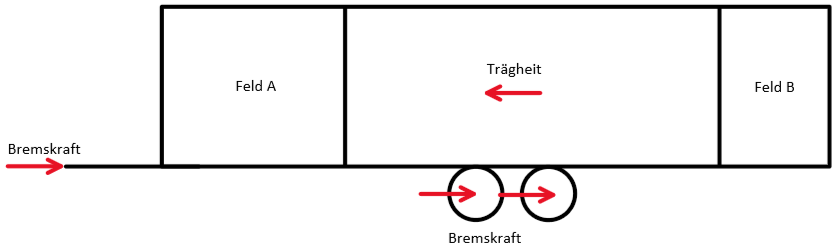
\includegraphics[width=0.8\textwidth]{04_Figures/1.2 Idealisierung.png}
    \captionof{figure}{Schematische darstellung der Kräfte während der longitudinalen Beschleunigung}
    \label{1.2 Idealisierung}
  \end{center}

  \paragraph{Kräfte und Spannungen}\mbox{}\\
  Die idealisierten Felder A und B und deren Lagerreaktionen und Schubkräfte sind in der Abbildung \ref{1.2 Felder} dargestellt. Die Kraft $F_a$ und $F_b$ ergeben sich aus der Masse des Aufbaus und der herrschenden Beschleunigung. Um die Berechnung zu vereinfachen werden die Lasteinleitungen jeweils in eine obere Ecke des Feldes gesetzt und entsprechend dem Hebelgesetz skaliert.

  \begin{figure}[!ht]
    \centering
      \begin{subfigure}[b]{0.5\textwidth}
         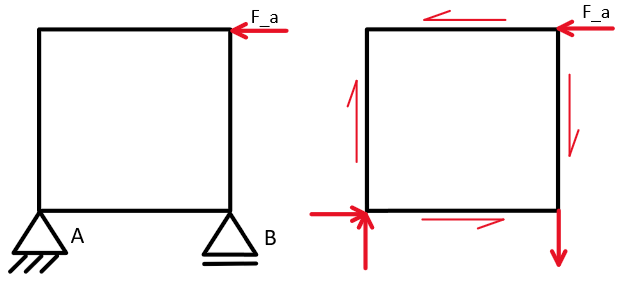
\includegraphics[width=1\linewidth]{04_Figures/1.2 Feld A}
         \caption{Feld A}
         \label{Feld A}
      \end{subfigure}
      \begin{subfigure}[b]{0.5\textwidth}
         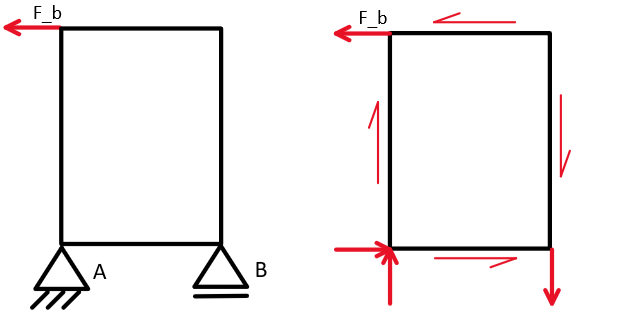
\includegraphics[width=1\linewidth]{04_Figures/1.2 Feld B}
         \caption{Feld B}
         \label{Feld B}
      \end{subfigure}
    \caption{Idealisierte Seitenwände, angreifende Käfte und Lagerreaktionen}
    \label{1.2 Felder}
  \end{figure}

  Bei einer Beschleunigung von 0.7 g ergeben sich Schubspannungen von 1.6 $\frac{N}{mm}$ im Feld A, sowie 2.8 $\frac{N}{mm}$ im Feld B. Die Normalkräfte in den umrahmenden Profilen im Feld A belaufen sich auf maximal 3.9 kN in den horizontalen, und auf 3.1 kN in den vertikalen Profilen. Im Feld B belaufen sich die Normalkräfte auf maximal 5.6 kN in den vertikalen, sowie 4.2 kN in den horizontalen Profilen.


\subsection{Laterale Beschleunigung}
\label{1.4 Laterale Beschleunigung}
  \paragraph{Idealisierung}\mbox{}\\
  Für den Lastfall \emph{1.4 lateralen Beschleunigung} wird der Solar Butterfly wie im Kapitel \ref{1.1 Vertikale Beschleunigung} als Biegebalken idealisiert. Da davon ausgegangen wird, dass sich der Schwerpunkt des Solar Butterflys auf einer ähnlichen Höhe wie der Flächenschwerpunk des idealisierten Querschnittes befindet, wird vereinfacht angenommen, dass die lateralen Trägheitskräfte im Flächenschwerpunk angreifen. (Vgl. Abbildung \ref{1.4 Idealisierter Querschnitt}) Auf diese weise kommt es zu keiner Verdrehung des Biegebalkens.\\
  Die Lagerung des idealisierten Solar Butterflys ist in der Abbildung \ref{1.4 Lagerung} dargestellt. Sie stellt die Ansicht von Oben auf den Solar Butterfly dar wobei der ``Spitz'' auf de linken Seite die Deichsel räpresentiert.

  \begin{figure}[!ht]
    \centering
      \begin{subfigure}{.5\textwidth}
        \centering
        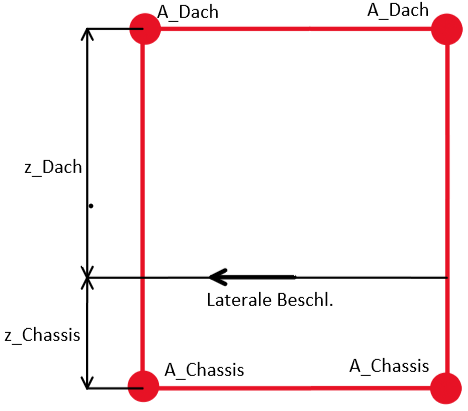
\includegraphics[width=0.8\linewidth]{04_figures/1.4 Querschnitt.png}
        \caption{Idealisierter Querschnitt}
        \label{1.4 Idealisierter Querschnitt}
      \end{subfigure}%
      \begin{subfigure}{.5\textwidth}
        \centering
        \includegraphics[width=0.75\linewidth]{04_figures/1.4 Träger.png}
        \caption{Schematische darstellung der idealisierung eines Trägers}
        \label{1.4 Träger}
      \end{subfigure}%
    \caption{Idealisierungen des Solar Butterflys für den Lastfall der lateralen Beschleunigung}
  \label{1.4 Idealisierung}
  \end{figure}

  Weiter wird angenommen, dass die Trägheitskräfte des Aufbaus über die Träger A und B auf das Chassis abgetragen werden. Wird angenommen, dass die Masse über die Höhe des Aufbaus gleichmässig verteilt ist, können die Trägheitskräfte als Streckenlasten, welche auf die Träger A und B wirken, idealisiert werden. Die vier Profile der Träger A und B müssen demnach je ein Viertel der Kräfte auf das Chassis übertragen. Die Idealisierung eines Trägers ist schematisch in der Abbildung \ref{1.4 Träger} dargestellt.\\
  Hierbei muss angemerkt werden, dass es sich um eine eher konservative Idealisierung handelt und die erhaltenen Kräfte und Spannunge zu hoch liegen werden. In dieser Idealisierung werden die in der Realität mittragenden Wände zwischen den Trägern, sowie die abschliessenden Wände im Kopf und am Heck nicht berücksichtigt. Dem zufolge ist auch die Annahme, dass ein Träger je ein Viertel der Trägheitskräfte auf das Chassis übertragen soll, eher unrealistisch. Die Berechnung wurde dennoch durchgeführt, um ein gefühl für die Grössenordnung der herrschenden Belastung zu erlangen.

  \begin{center}
    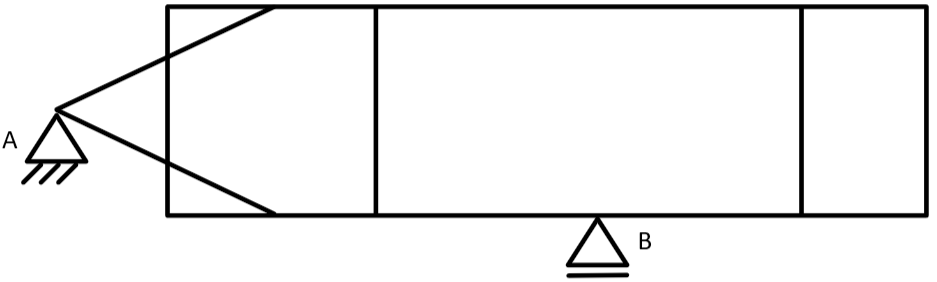
\includegraphics[width=0.6\textwidth]{04_Figures/1.4 Lagerung.png}
    \captionof{figure}{Lagerung des idealisierten Solar Butterfly}
    \label{1.4 Lagerung}
  \end{center}

  \paragraph{Querkraft- und Biegemomentenverlauf - Biegebalken}\mbox{}\\
  Aus der Massenverteilung und der Beschleunigung können die Lagerreaktionen sowie die Trägheitskräfte berechnet werden. Der daraus resultierende Querkraft- und Biegemomentenverlauf ist in der Abbildung \ref{1.4 QM} dargestellt.

  \begin{figure}[!ht]
    \centering
      \begin{subfigure}{.5\textwidth}
        \centering
        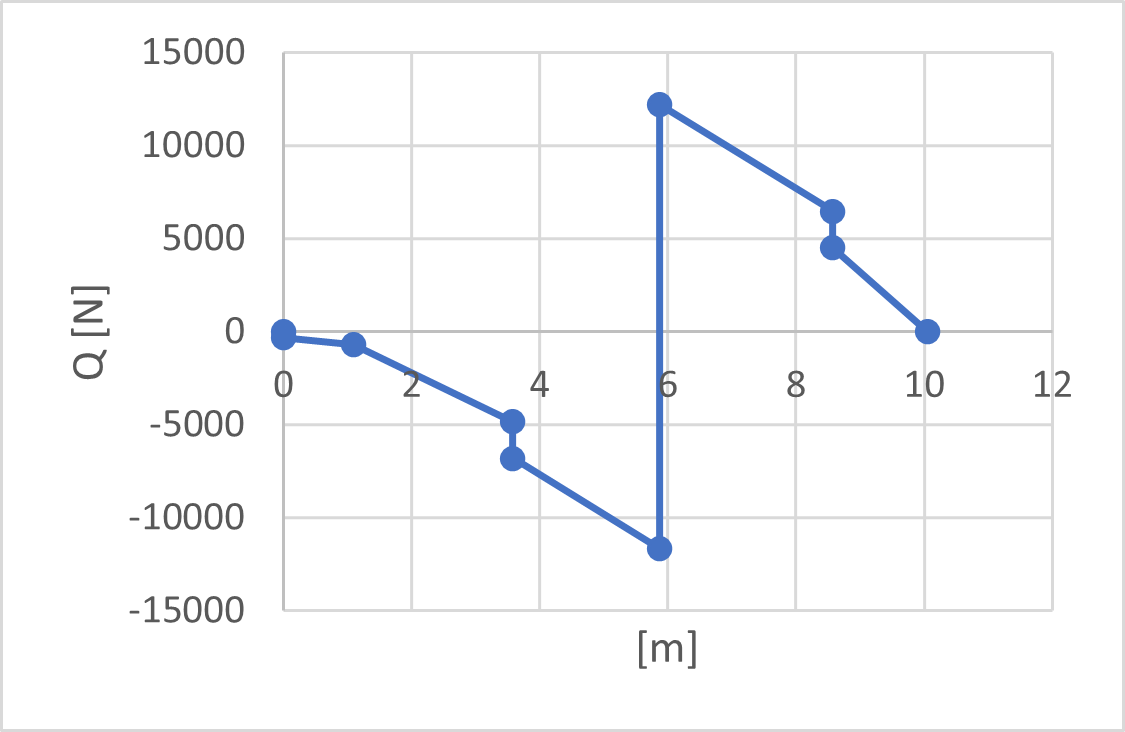
\includegraphics[width=.98\linewidth]{04_figures/1.4 Q.png}
        \caption{Querkraftverlauf}
        \label{1.4 Q}
      \end{subfigure}%
      \begin{subfigure}{.5\textwidth}
        \centering
        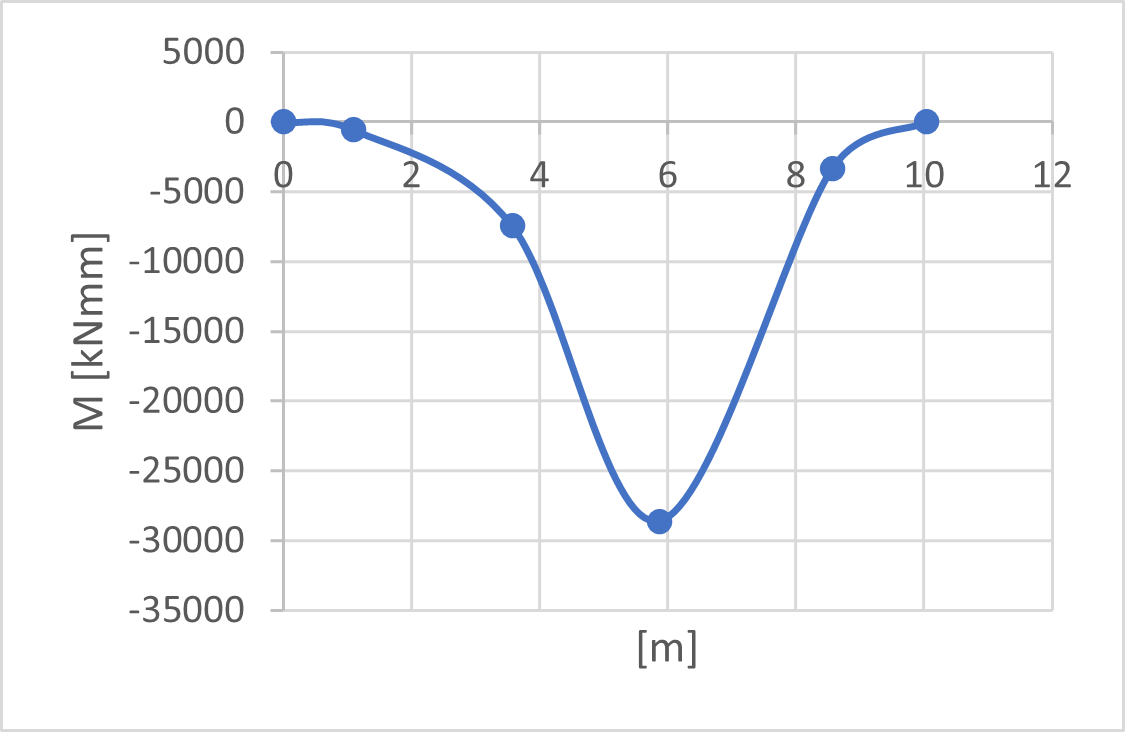
\includegraphics[width=.98\linewidth]{04_figures/1.4 M.png}
        \caption{Biegemomentenverlauf}
        \label{1.4 M}
      \end{subfigure}%
    \caption{Querkraft- und Biegemomentenverlauf des als Biegebalken idealisierten Solar Butterfly im Lastfall der lateralen Beschleunigung}
  \label{1.4 QM}
  \end{figure}

  \paragraph{Kräfte und Spannungen}\mbox{}\\
  Die Kräfte und Spannungen werden analog zum Kapitel \ref{1.1 Vertikale Beschleunigung} \emph{Vertikale Beschleunigung} berechnet. Bei einem Maximalen Biegemoment von 29'000 kNmm ergeben sich Spannungen von 7 MPa im Chassis, sowie 2.3 MPa in den Dachträgern. Sie entsprechen Kräften von 11.4 kN, respektive 0.9 kN. Der maximale Schubfluss infolge der Querkraft ergibt sich zu 2.65 $\frac{N}{mm}$

  \paragraph{Spannungen in den Trägern}\mbox{}\\
  Aus der Masse des Aufbaus, der wirkenden Beschleunigung und der Höhe des Profiles kann die Streckenlast pro Träger ermittelt werden, woraus wiederrum der Querkraft- und Biegemomentenverlauf bestimmt werden kann. Dieser ist in der Abbildung \ref{1.4 QM} dargestellt. Mit dem angenommenen Trägerprofil (vgl. Kapitel KAPITEL) ergeben sich maximale an Spannungen an der Einspannung von 15 MPa.

  \begin{center}
    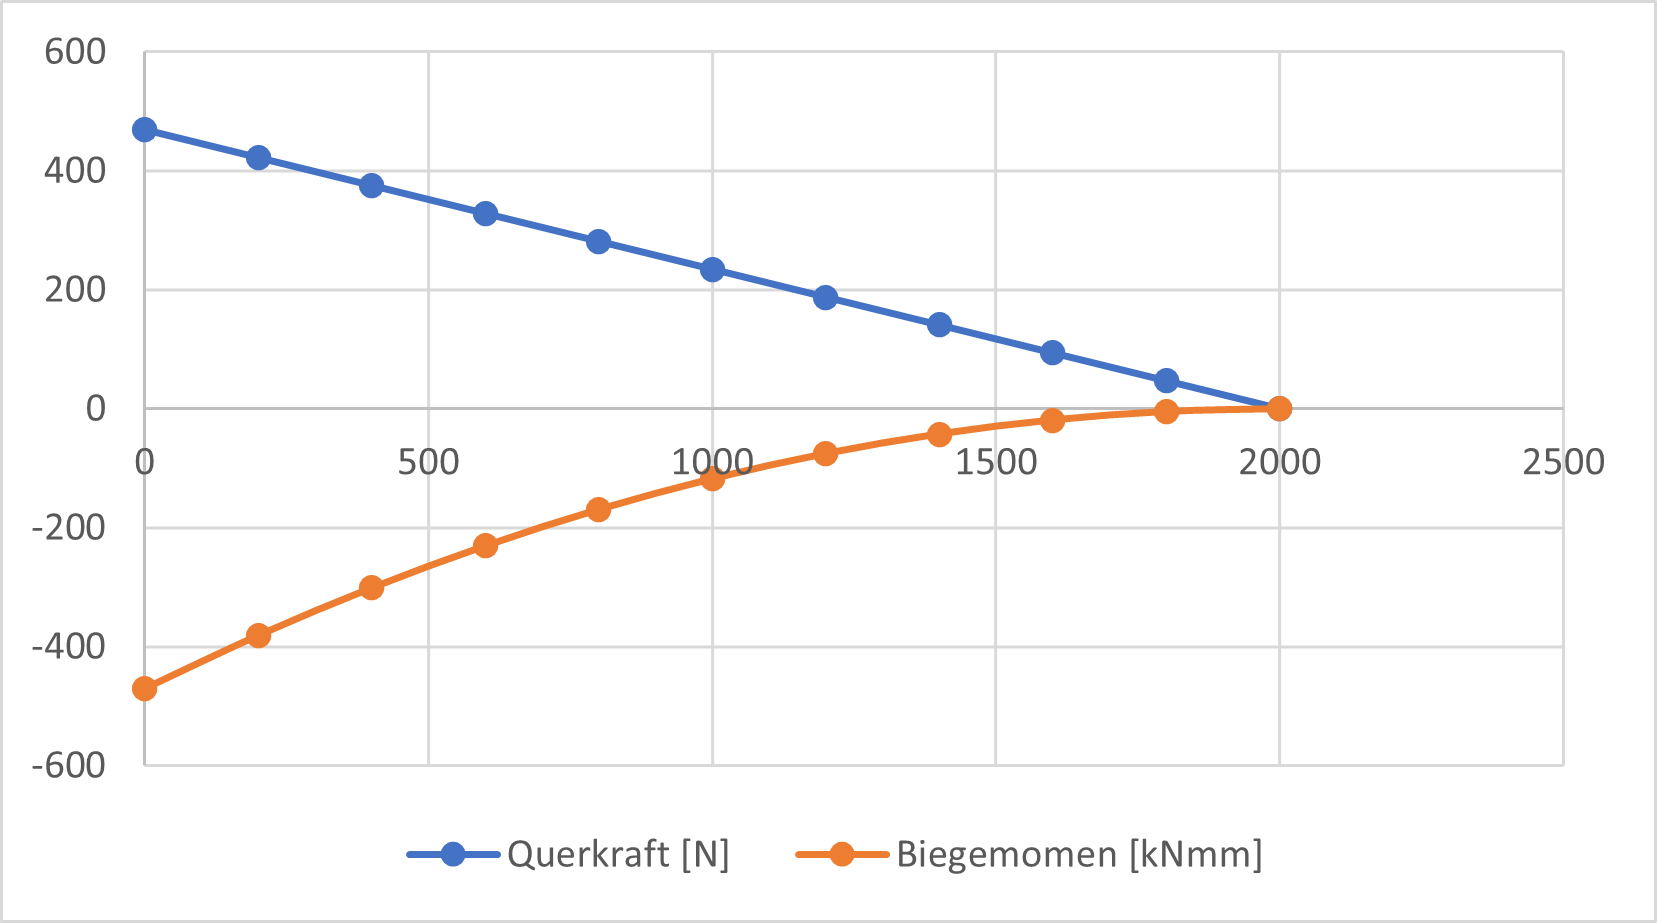
\includegraphics[width=0.7\textwidth]{04_Figures/1.4 QM.png}
    \captionof{figure}{Querkraft und Biegemomentenverlauf in den Profilen der Träger im Lastfall der lateralen Beschleunigung}
    \label{1.4 QM}
  \end{center}




\subsection{Rotatorische Beschleunigung}
\label{1.5 Rotatorische Beschleunigung}
\paragraph{Idealisierung}\mbox{}\\
Um die Schubflüsse in den Wänden des Solar Butterflys, entstehend aus der rotatorischen Beschleunigung, berechnen zu können, wird der Solar Butterfly idealisiert als Torsionsbalken betrachtet. Das Kräftegleichgewicht der Idealisierung ist der Abbildung \ref{1.5 Idealisierung} zu entnehmen. Um auf das Torsionsmoment, welches nötig ist um die rotatorische Beschleunigung aus dem Lastfall \emph{1.5 Rotatorische Beschleunigung} zu erreichen, schliessen zu können, wird das Massenträgheitsmoment berechnet. Dabei wird der Solar Butterfly in die beiden Bereiche \emph{Chassis} und \emph{Aufbau} aufgeteilt (Vgl. Abbildung \ref{1.5 Idealisierung}). Es wird vereinfacht angenommen, dass die Masse des jeweiligen Bereiches auf dessen Querschnittsfläche homogen verteilt ist. Dank dieser Annahme lässt sich das Massenträgheitsmoment, unter berücksichtigung des Satzes von \emph{Steiner}, wie folgt berechnen.

\begin{equation}
  I_{rot} = \frac{1}{12} \cdot m \cdot \left(H\ddot{o}he^2 + Breite^2\right) + m \cdot r^2
\end{equation}

Das Torsionsmoment ergibt sich aus folgendem Zusammenhang:
\begin{equation}
  M_t = I_{rot} \cdot \alpha
\end{equation}

\begin{center}
  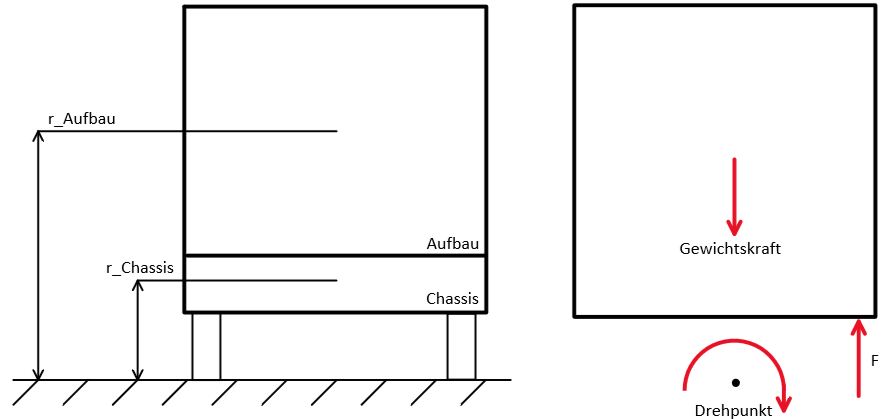
\includegraphics[width=0.7\textwidth]{04_Figures/1.5 Idealisierung.png}
  \captionof{figure}{Schematische Darstellung des Solar Butterflys für den Lastfall der rotatorischen Beschleunigung}
  \label{1.5 Idealisierung}
\end{center}

\paragraph{Berechnung}\mbox{}\\
Bei einem Massenträgheitsmoment von rund 8700 $kg\;m^2$ resultiert ein Torsionsmoment von 38'400 $kNmm$. Wird dies nun in die Kraft $F$ (vgl. Abbildung \ref{1.5 Idealisierung}) umgerechnet, ergibt sich eine Kraft von ca. 43 kN. Als Vergleich dazu steht die Kraft von von 37 kN, welche aus der vertikalen Beschleunigung von 2.5 g (Lastfall \emph{1.1 Vertikale Beschleunigung} + Erdbeschleunigung) entsteht.

Um die aus dem Torsionsmoment resultierende Schubflüsse zu berechnen, wird der Solar Butterfly, gemäss Abbildung \ref{1.5 Momente}, in vier Abschnitte eingeteilt. Ebenfalls in dieser Abbildung dargestellt ist das schematisch dargestellte angreifende Torsionsmoment (schwarzer Pfeil) und die aus der Trägheit resultierenden Reaktionsmomente (rote Pfeile). Für jeden dieser vier Abschnitte wird, unter berücksichtigung der Massenverteilung, das Massenträgheitsmoment berechnet, um auf den Momentenverlauf schliessen zu können, welcher in der Abbildung \ref{1.5 Momentenverlauf} dargestellt ist.

\begin{center}
  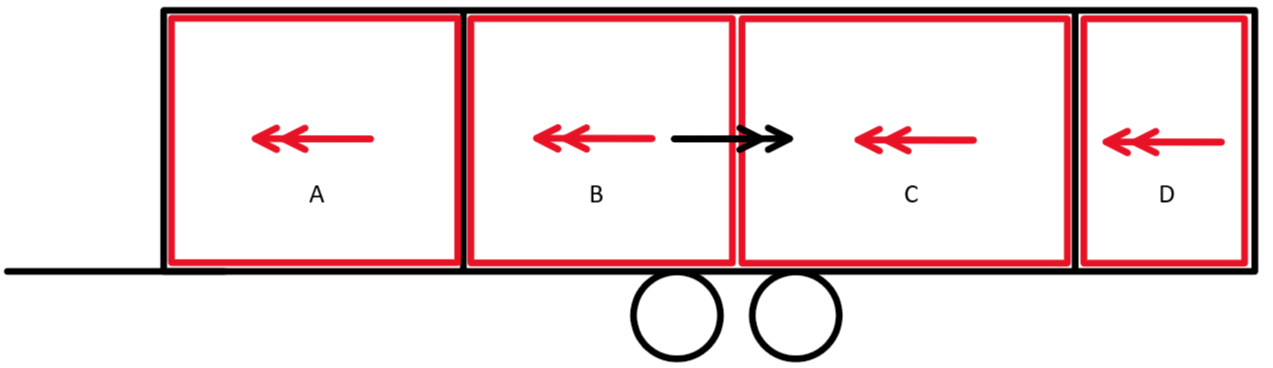
\includegraphics[width=0.8\textwidth]{04_Figures/1.5 Momente.png}
  \captionof{figure}{Schematische Darstellung des Solar Butterflys für den Lastfall der rotatorischen Beschleunigung}
  \label{1.5 Momente}
\end{center}

\begin{center}
  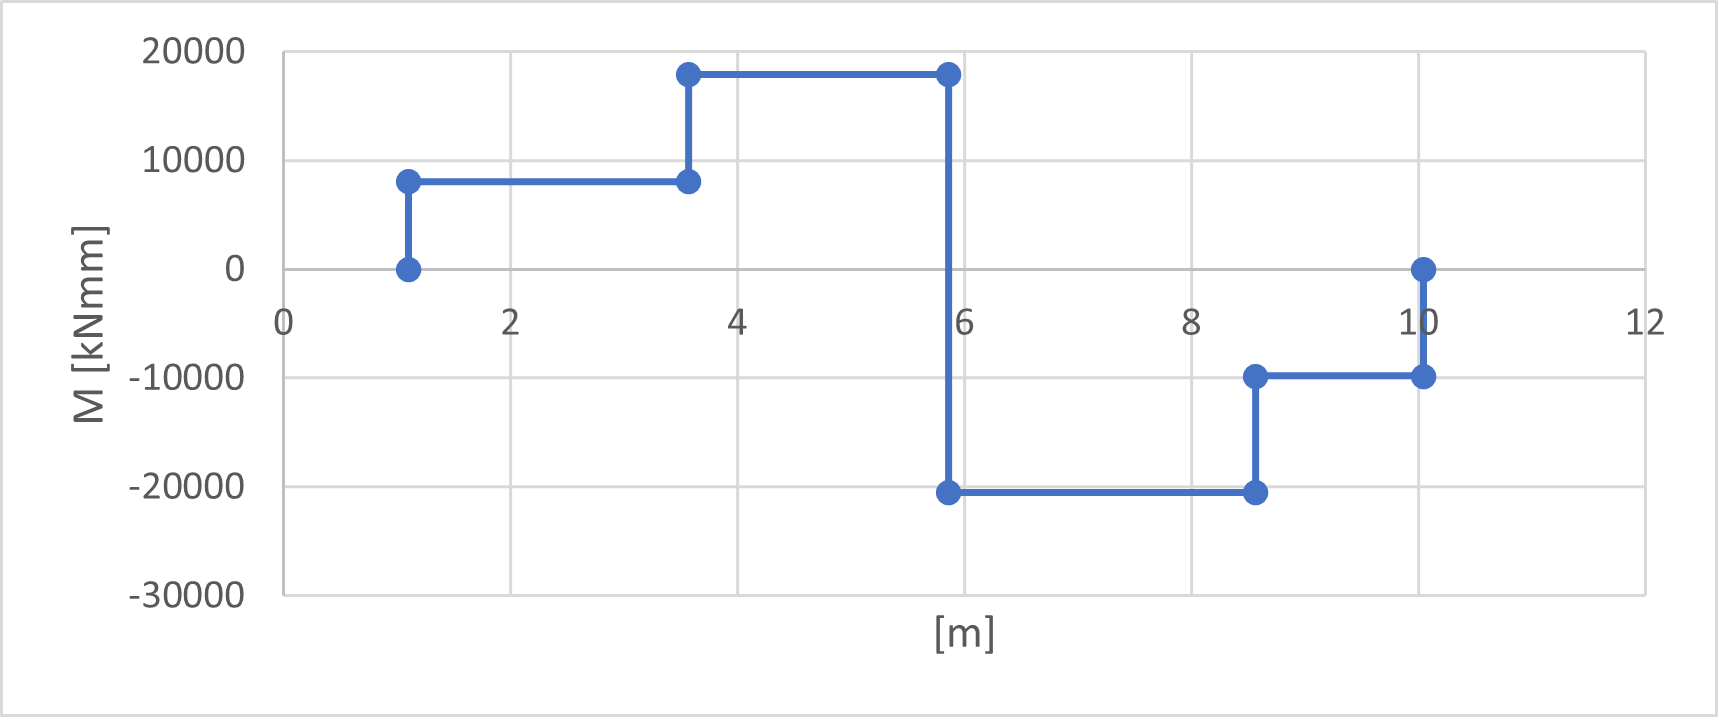
\includegraphics[width=0.8\textwidth]{04_Figures/1.5 Momentenverlauf.png}
  \captionof{figure}{Torsionsmomentenverlauf für den Lastfall der rotatorischen Beschleunigung}
  \label{1.5 Momentenverlauf}
\end{center}

Ahnand der Torsionsmomente pro Abschnitt kann wiederum die Schubflüsse geschlossen werden, welche mit der Formel \ref{Schubfluss} berechnet werden können.

\begin{equation}
  q = \frac{M_t}{2 \cdot A_m}
  \label{Schubfluss}
\end{equation}

Wobei $A_m$ für die Bred'sche Fläche steht.
Die Schubflüsse und Momente je Abschnitt können aus der Tabelle \ref{Schubfluss resultat} entnommen werden.


\begin{table}[h!]
  \centering
  \begin{tabular}{ccc}
    \thickhline
    Feld & Torsionsmoment [kNmm] & Schubfluss [N/mm] \\ \hline
    A    & 8047                  & 0.81\\
    B    & 9880                  & 1.00\\
    C    & 10706                 & 1.08\\
    D    & 9811                  & 0.99\\
    \thickhline
  \end{tabular}
\caption{Torsionsmomente und Schubflüsse entstehend aus der rotatorischen Beschleunigung}% Add 'table' caption
\label{Schubfluss resultat}
\end{table}

\newpage



















% \section{Komponenten und Verbindungen}
% In diesem Kapitel wird beschrieben, wie der Solar Butterfly aufgebaut ist. Es werden verschiedene Komponenten eingeführt und analysiert wie diese Komponenten miteinander Verbunden sind und welche Kräfte die Verbindungen übertragen müssen.\\
% Weiter wird beschrieben, wie der SB vereinfacht betrachtet wird (Biegebalken) in zwei Moden. (A und C)
%
% \subsection{Komponenten}
% bla bla
%
% \paragraph{Hauptkörper}
% Ganzer Körper als einen Kasten betrachten
% \begin{description}
%   \item \textbf{Chassis}\\
%   Idealisierung: Beam
%   \item \textbf{Boden}\\
%   Auslegung: Biegebalken
%   Idealisierung: Schalenkörper\\
%   \item \textbf{Stützen A und B}\\
%   Auslegung: Schubwand mit Türe\\
%   Profile nehmen Kräfte auf, geben diese Jedoch an die Schubwand weiter\\
%   \item \textbf{Dach}\\
%   Panelen: Schubfläche\\
%   Dach an sich: Biegebalken (Durch eigengewicht)
%   Im Modus \emph{C} Kräfte auf nehmen durch Verriegelung der Seitenwände
% \end{description}
%
% \paragraph{Seitenmodul}
% \begin{description}
%   \item \textbf{Boden}\\
%   Biegebalken und Schubfläche
%   \item \textbf{Seitenwand}\\
%   Modus A: Schubwand\\
%   Modus C: Keine
%   \item \textbf{Ausfahrmechanismus (Scharniere)}\\
%   Wand: Schubwand
%   \item \textbf{}\\
%   \item \textbf{}\\
% \end{description}
